\chapter{Application Interfaces}

This chapter presents the realized user interfaces of the Predictra Threat Map platform. The application is built using React and styled with a custom dark-mode theme designed for security operations centers, prioritizing high contrast and minimal visual fatigue.

\section{Live Threat Map}
The primary interface is the 3D globe visualization. As threats are ingested by the backend scrapers, they are streamed via Server-Sent Events to the frontend, which renders them as dynamic arcs and pulsating markers on the interactive Earth canvas.

\begin{figure}[H]
    \centering
    
\includegraphics[width=\textwidth]{assets/screenshots/live_map.png}
    \caption[The 3D Live Threat Map.]{The 3D Live Threat Map showing active threat corridors and origin/destination coordinates.}
    \label{fig:ui_livemap}
\end{figure}

\section{System Dashboard}
The Dashboard provides an immediate overview of the system's operational health, ingestion rates, and recent high-severity alerts. It acts as the tactical command center for security engineers.

\begin{figure}[H]
    \centering
    
\includegraphics[width=\textwidth]{assets/screenshots/dashboard.png}
    \caption[The System Dashboard.]{The System Dashboard displaying active feed metrics and high-severity threat summaries.}
    \label{fig:ui_dashboard}
\end{figure}

\section{STIX Intelligence Workspace}
The STIX (Structured Threat Information Expression) dashboard allows investigators to upload JSON threat bundles. The system maps the parsed entities to the MITRE ATT\&CK kill chain.

\begin{figure}[H]
    \centering
    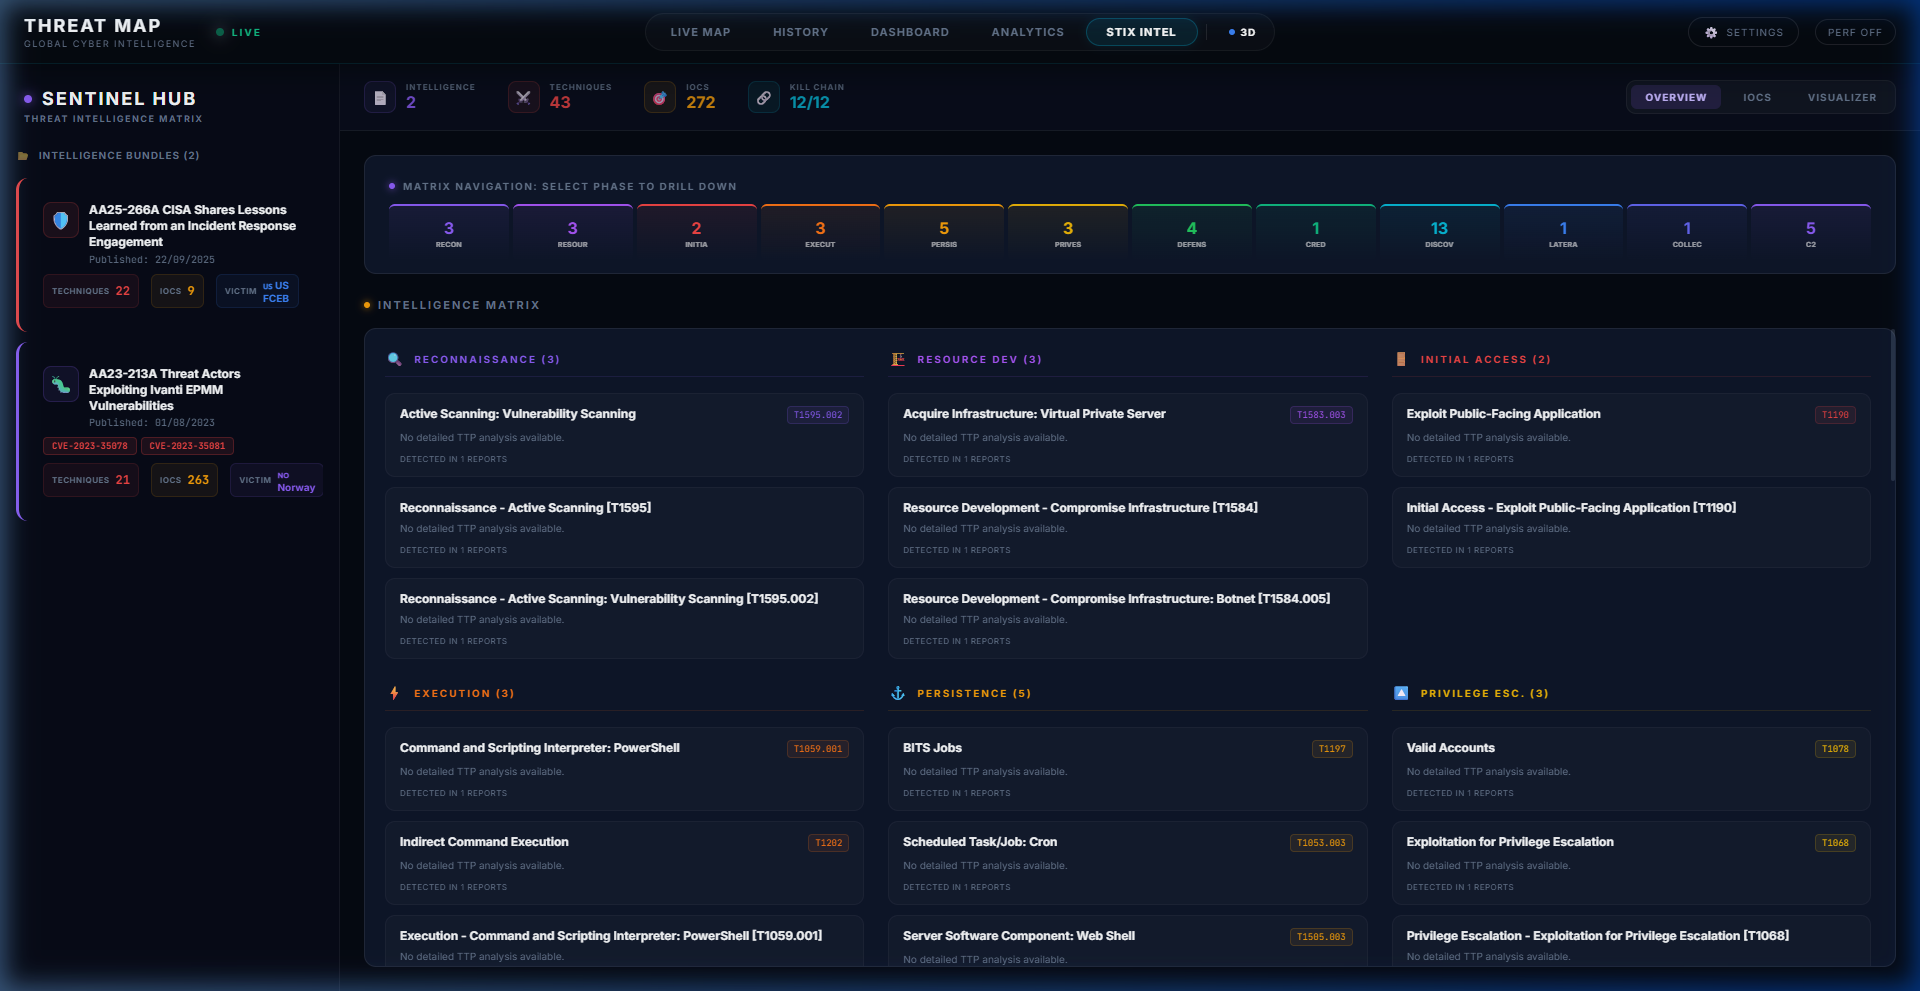
\includegraphics[width=\textwidth]{assets/screenshots/stix.png}
    \caption[The STIX 2.1 Workspace.]{The STIX 2.1 Workspace displaying an uploaded threat bundle.}
    \label{fig:ui_stix}
\end{figure}

\section{Historical Threat Browser}
To investigate past campaigns, the History tab provides a paginated view into the MongoDB Atlas logs. Analysts can execute complex queries, filter by target industry or malware family, and export the filtered results.

\begin{figure}[H]
    \centering
    
\includegraphics[width=\textwidth]{assets/screenshots/history.png}
    \caption[The Historical Threat Browser.]{The Historical Threat Browser with paginated data tables and advanced filtering capabilities.}
    \label{fig:ui_history}
\end{figure}

\section{Global Analytics}
The Analytics interface tracks long-term trends and adversary behaviors. It aggregates the ingested threat logs to display statistical distributions of malware types, top targeted countries, and active sectors.

\begin{figure}[H]
    \centering
    
\includegraphics[width=\textwidth]{assets/screenshots/analytics.png}
    \caption[The Analytics Dashboard.]{The Analytics Dashboard presenting aggregate threat metrics and sector distributions.}
    \label{fig:ui_analytics}
\end{figure}
